\documentclass[11pt, a4paper]{article}
\usepackage[english]{babel}
\usepackage[utf8]{inputenc}
\usepackage{fancyhdr}
\usepackage{lastpage}
\usepackage{datetime}
\usepackage{indentfirst}
\usepackage{hyperref}
\usepackage{appendix}
\usepackage{amsmath}
\usepackage{amssymb}
\usepackage{amsfonts}
\usepackage{mathtools}
\usepackage{siunitx}
\usepackage{cancel}
\usepackage{tabularray}
\usepackage{multirow}
\usepackage{array}
\usepackage{hhline}
\usepackage{makecell}
\usepackage{courier}
\usepackage[font=small, skip=0pt]{caption}
\usepackage[font=scriptsize, skip=0pt]{subcaption}
\usepackage{float}
\usepackage{graphicx}
\usepackage{listings}
\usepackage{xcolor}
\usepackage{matlab-prettifier}
\usepackage[T1]{fontenc}
\usepackage{lmodern}
\usepackage{bigfoot}
\usepackage{filecontents}
\usepackage[nottoc]{tocbibind}

\graphicspath{ {./mathimages/} }

\newdateformat{Datea}{\THEDAY\ \monthname[\THEMONTH] \THEYEAR}
\newdateformat{Dateb}{\monthname[\THEMONTH] \THEYEAR}

%\allowdisplaybreaks
\DeclareMathOperator{\cosec}{cosec}
\DeclareMathOperator{\cotan}{cotan}
\DeclareMathOperator{\sech}{sech}
\DeclareMathOperator{\cosech}{cosech}
\DeclareMathOperator{\arcsec}{arcsec}
\DeclareMathOperator{\arccot}{arccot}
\DeclareMathOperator{\arccsc}{arccosec}
\DeclareMathOperator{\arccosh}{arccosh}
\DeclareMathOperator{\arcsinh}{arcsinh}
\DeclareMathOperator{\arctanh}{arctanh}
\DeclareMathOperator{\arcsech}{arcsech}
\DeclareMathOperator{\arccsch}{arccsch}
\DeclareMathOperator{\arccoth}{arccoth}
\DeclareMathOperator{\arsinh}{arsinh}
\DeclareMathOperator{\arcosh}{arcosh}
\DeclareMathOperator{\artanh}{artanh}

\DeclareMathOperator{\cis}{cis}

\pagestyle{fancy}
\fancyhf{}
\rhead{Hatam Barma}
\chead{\begin{tabular}[t]{@{}l@{}}\\Mathematics and Further Mathematics Pure Revision Summary\end{tabular}}
\lhead{\Dateb\today}
\cfoot{Page \thepage}

\renewcommand{\thesection}{\arabic{section}} 

\renewcommand{\thesubsection}{\thesection.\arabic{subsection}}

\setcounter{section}{4}

\allowdisplaybreaks

\fancypagestyle{plain}{
\fancyhf{}
\renewcommand{\headrulewidth}{0pt}}

\hypersetup{
    colorlinks,
    citecolor=black,
    filecolor=black,
    linkcolor=blue,
    urlcolor=magenta!70!black
}

\begin{document}


\begin{titlepage}
   \begin{center}
       \vspace*{2.5cm}
	\huge
       \textbf{A-Level Mathematics and Further Mathematics Pure Revision Summary} \\
	\vspace{1cm}
	\Large
       \textbf{Chapter 5: Vectors and Matrices}
            
       \vspace{1.5cm}
	\LARGE
       \textbf{Hatam Barma} \\
	\vspace{0.75cm}
       \normalsize
       \emph{Compiled on \Datea\today} \\

       \vfill
        

	E-mail: hatam.barma@gmail.com
   \end{center}
\end{titlepage}


\tableofcontents

\clearpage
\section{Vectors and Matrices}
\vspace{0.5cm}

\subsection{Vector notation}
\begin{itemize}
\item A Level M AS / Year 1 \hspace{1cm} \phantom{ } Pages 220 -- 244
\end{itemize} \par
An arrow above two letters, such as
\begin{equation*}
\overrightarrow{AB}
\end{equation*}
 denotes the vector that takes point $A$ to point $B$. Also note:
\begin{equation*}
\overrightarrow{AB}+\overrightarrow{BC}=\overrightarrow{AC}
\end{equation*}
The vector ascribed to a variable, for example $r$ can be shown to be a vector quantity in three ways. When in print, vectors are commonly denoted in bold. However it is quite hard to handwrite bold font. So, we can either underline the character, or put an arrow over the top. All three are equivalent ways of writing the same vector quantity.


\begin{figure}[H]
\centering
\begin{subfigure}[c]{0.59\textwidth}
\begin{center}
\begin{tblr}{|[.75pt]|c|c|c||[.75pt]}
\hline[1.25pt]
Bold font & Underline & Arrow \\ \hline
$\boldsymbol{r}$ & $\underline{r}$ & $\vec{r}$ \\ \hline[1pt]
\end{tblr}
\end{center}
\end{subfigure}
\hfill
\begin{subfigure}[c]{0.39\textwidth}
\centering
\begin{equation*}
\boldsymbol{r} = \underline{r} = \vec{r} = \begin{bmatrix}x\\y\\z\end{bmatrix}
\end{equation*}
\end{subfigure}
\end{figure}
\begin{itemize}
\item[Note:] Normalised vectors (vectors of length 1) are often written with a `hat' above them
\end{itemize}
\begin{gather*}
\hat{\boldsymbol{r}}=\hat{\underline{r}}=\hat{\vec{r}}=\frac{1}{\sqrt{x^{2}+y^{2}+z^{2}}}\begin{bmatrix}x\\y\\z\end{bmatrix} \\
\boldsymbol{r}=|\boldsymbol{r}|\hat{\boldsymbol{r}} \hspace{1.5cm} \hat{\boldsymbol{r}}=\frac{1}{|\boldsymbol{r}|}\boldsymbol{r}
\end{gather*}
\vspace{0.5cm}


\subsection{The vector equation of a line}
\begin{itemize}
\item A Level FM AS / Year 1 \hspace{1cm} Pages 33 -- 39
\item A Level FM AS / Year 1 \hspace{1cm} Pages 45 -- 48
\end{itemize} \par
A line can be defined in terms of vectors or Cartesian coordinates. the form
\begin{equation*}
\boldsymbol{r}=\boldsymbol{a}+\lambda\boldsymbol{b}
\end{equation*}
gives the position vector of a point on the line, where
\begin{itemize}
\item[-]$\boldsymbol{a}$ is the position vector of a fixed point on the line
\vspace{-0.25cm}
\item[-]$\boldsymbol{b}$ is the vector which maps $\boldsymbol{a}$ to another point on the line
\vspace{-0.25cm}
\item[-]$\boldsymbol{r}$ is a general point on the line
\vspace{-0.25cm}
\item[-]$\lambda$ is a scalar variable coefficient
\end{itemize}

In 2D, lines must be either \underline{parallel}, or \underline{intersecting}, unless they are the same line.

In 3D, lines can be either \underline{parallel}, or \underline{non-parallel and intersecting}, or \underline{non-parallel and non-intersecting} (skew), unless they are the same line.
\vspace{0.5cm}


\subsection{Cartesian form of the equations of a line in 3D}
\begin{itemize}
\item A Level FM AS / Year 1 \hspace{1cm} Pages 39 -- 45
\end{itemize} \par
A line can also be defined in terms of Cartesian coordinates. This can be done by rearranging the vector equation.
\begin{equation*}
\begin{bmatrix}x\\y\\z\end{bmatrix}=\boldsymbol{r}=\begin{bmatrix}a\\b\\c\end{bmatrix}+\lambda\begin{bmatrix}f\\g\\h\end{bmatrix}
\end{equation*}
\begin{flalign*}
\Rightarrow x&=a+f\lambda & \hspace{-1cm}\Leftrightarrow \hspace{1cm}& \lambda=\frac{x-a}{f} && \\
\Rightarrow y&=b+g\lambda & \hspace{-1cm}\Leftrightarrow \hspace{1cm}& \lambda=\frac{y-b}{g} && \\
\Rightarrow z&=c+h\lambda & \hspace{-1cm}\Leftrightarrow \hspace{1cm}& \lambda=\frac{z-c}{h} &&
\end{flalign*} \newline \par
Therefore, the Cartesian form of the line is
\begin{equation*}
\frac{x-a}{f}=\frac{y-b}{g}=\frac{z-c}{h}(=\lambda)
\end{equation*}
This form can be easily rearranged to give $x$, $y$, and $z$ in terms of $\lambda$, from which the vector equation may be obtained.
\vspace{0.5cm}

\newpage
\subsection{The scalar product (or dot product)}
\begin{itemize}
\item A Level FM AS / Year 1 \hspace{1cm} Pages 48 -- 56
\end{itemize} \par
The scalar product of two vectors is an operation which takes two vectors and returns a scalar, hence the name `scalar' product. This `derivation' is not necessary to remember, but the final result is an important one.
\begin{figure}[H]
\centering
\begin{subfigure}[b]{0.85\textwidth}
\scalebox{.85}{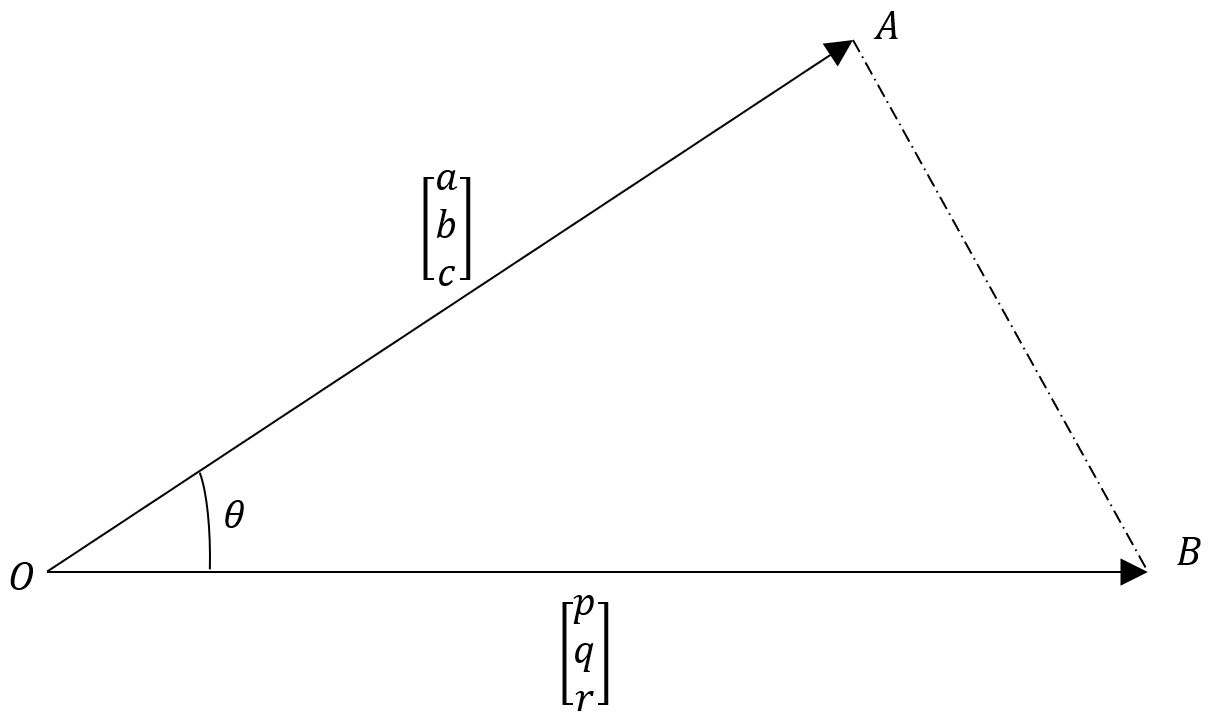
\includegraphics[width=\textwidth]{scalarproduct}}
\end{subfigure}
\end{figure}
Using the cosine rule, we obtain:
\begin{equation*}
\left( \overrightarrow{AB} \right)^{2}=\left( \overrightarrow{OA} \right)^{2}+\left( \overrightarrow{OB} \right)^{2}-2\cdot\left( \overrightarrow{OA} \right)\cdot\left( \overrightarrow{OB} \right)\cdot\cos(\theta)
\end{equation*}

And,
\begin{equation*}
\overrightarrow{AB}=\overrightarrow{OB}-\overrightarrow{OA}=\begin{bmatrix} p-a \\ q-b \\ r-c \end{bmatrix}
\end{equation*}

Therefore:
\begin{equation*}
\begin{bmatrix} p-a \\ q-b \\ r-c \end{bmatrix}^{2}=\begin{bmatrix} a \\ b \\ c \end{bmatrix}^{2}+\begin{bmatrix} p \\ q \\ r \end{bmatrix}^{2}-2\begin{bmatrix} a \\ b \\ c \end{bmatrix}\begin{bmatrix} p \\ q \\ r \end{bmatrix}\cos(\theta)
\end{equation*}

We can expand this, by taking the magnitude (represented by $|\cdot|$) of each of the vectors involved:
\small
\begin{multline*}
(p-a)^{2}+(q-b)^{2}+(r-c)^{2}=\\ \left( a^{2} +b^{2} +c^{2} \right) + \left( p^{2} +q^{2} +r^{2} \right) - 2\sqrt{ a^{2} +b^{2} +c^{2}}\sqrt{ p^{2} +q^{2} +r^{2}}\cos(\theta)
\end{multline*}
\begin{multline*}
p^{2}-2ap+a^{2}+q^{2}-2qb+b^{2}+r^{2}-2cr+c^{2}=\\a^{2}+b^{2}+c^{2}+p^{2}+q^{2}+r^{2}-2\sqrt{ a^{2} +b^{2} +c^{2}}\sqrt{ p^{2} +q^{2} +r^{2}}\cos(\theta)
\end{multline*}
\begin{multline*}
\cancel{p^{2}}+\cancel{a^{2}}+\cancel{q^{2}}+\cancel{b^{2}}+\cancel{r^{2}}+\cancel{c^{2}}-2(ap+bq+cr)=\\\cancel{a^{2}}+\cancel{b^{2}}+\cancel{c^{2}}+\cancel{p^{2}}+\cancel{q^{2}}+\cancel{r^{2}}-2\sqrt{ a^{2} +b^{2} +c^{2}}\sqrt{ p^{2} +q^{2} +r^{2}}\cos(\theta)
\end{multline*}
\normalsize
Thus:
\begin{equation*}
\cos(\theta)=\frac{(ap+br+cq)}{\sqrt{ a^{2} +b^{2} +c^{2}}\sqrt{ p^{2} +q^{2} +r^{2}}}=\frac{(ap+br+cq)}{\left|\begin{bmatrix} a \\ b \\ c \end{bmatrix}\right|\times\left|\begin{bmatrix} p \\ q \\ r \end{bmatrix}\right|}
\end{equation*}
This rearranges to give
\begin{equation*}
\left|\begin{bmatrix} a \\ b \\ c \end{bmatrix}\right|\times\left|\begin{bmatrix} p \\ q \\ r \end{bmatrix}\right|\times \cos(\theta)=ap+br+cq
\end{equation*}

We can therefore define the \emph{scalar product}, or \emph{dot product} of two vectors $\boldsymbol{x}$ and $\boldsymbol{y}$ to be
\begin{equation*}
\boldsymbol{x}\cdot\boldsymbol{y}=\begin{bmatrix} a \\ b \\ c \end{bmatrix}\cdot\begin{bmatrix} p \\ q \\ r \end{bmatrix}=ap+bq+cr
\end{equation*}

$\boldsymbol{x}$ and $\boldsymbol{y}$ are both vectors, however their scalar product, denoted by a `dot', $(ap+bq+cr)$ is a scalar. The scalar product theorem is defined as:
\begin{equation*}
\boldsymbol{x}\cdot\boldsymbol{y}=|\boldsymbol{x}||\boldsymbol{y}|\cos(\theta)
\end{equation*}
An important result is that if the two vectors are perpendicular, the angle between them is $90^{\circ}$, and $\cos(90)=0$, so the scalar product is 0. On the other hand, if the two vectors are the same, then the angle between them is $0^{\circ}$, and $\cos(0)=1$, so the scalar product is the square of the magnitude of the vector.
\vspace{0.5cm}


\subsection{The vector product (or cross product)}
\label{crossproduct}
\begin{itemize}
\item A Level FM AS / Year 1 \hspace{1cm} Pages 56 -- 61
\end{itemize} \par
The vector product of two vectors is an operation which takes two vectors and returns another vector, which is perpendicular to both the original vectors. Again, the derivation is unnecessary to remember, but the final results are very important.\newline\par

We want to find
\begin{equation*}
\begin{bmatrix}x\\y\\z\end{bmatrix}\perp\begin{bmatrix}a\\b\\c\end{bmatrix},\begin{bmatrix}p\\q\\r\end{bmatrix}
\end{equation*}
From the scalar product theorem, for perpendicular vectors, we require
\begin{align*}
\begin{bmatrix}x\\y\\z\end{bmatrix}\cdot\begin{bmatrix}a\\b\\c\end{bmatrix}&=0 & \begin{bmatrix}x\\y\\z\end{bmatrix}\cdot\begin{bmatrix}p\\q\\r\end{bmatrix}&=0 \\
& & & \\
ax+by+cz&=0 & px+qy+rz&=0 \\
arx+bry+crz&=0 & pcx+qcy+rcz&=0
\end{align*}
Therefore:
\begin{flalign*}
(arx+bry+crz)-(pcx+qcy+rcz)&=0 && \\
(arx+bry-cpx-qcy)&=0 && \\
(ar-cp)x+(br-cq)y&=0 && \\
(br-cq)y&=-(ar-cp)x && \\
&=(cp-ar)x  &&
\end{flalign*}

Let $x=(br-cq)$ and let $y=(cp-ar)$. Substituting this back in,
\begin{flalign*}
a(br-cq)+b(cp-ar)+cz&=0 && \\
\cancel{abr}-acq+bcp-\cancel{bar}&=-cz && \\
c(bp-aq)&=-cz && \\
& && \\
z&=(aq-bp)
\end{flalign*}
So,
\begin{equation*}
\begin{bmatrix}x\\y\\z\end{bmatrix}=\begin{bmatrix}br-cq\\cp-ar\\aq-bp\end{bmatrix}
\end{equation*}
and so we define the cross product:
\begin{equation*}
\begin{bmatrix}a\\b\\c\end{bmatrix}\times\begin{bmatrix}p\\q\\r\end{bmatrix}=\begin{bmatrix}br-cq\\cp-ar\\aq-bp\end{bmatrix}
\end{equation*}

$\boldsymbol{x}$ and $\boldsymbol{y}$ are both vectors, and their vector product, denoted by a `cross', is a vector. The vector product theorem is defined as:
\begin{equation*}
\boldsymbol{x}\times\boldsymbol{y}=|\boldsymbol{x}||\boldsymbol{y}|\sin(\theta)
\end{equation*} 

There are a couple of tricks to remembering how the cross product evaluates. Here is one, but by no means the only way of doing it. \newline \par

\noindent Take the determinant of the $3\times3$ matrix:
\begin{equation*}
\begin{bmatrix} \hat{\boldsymbol{\imath}} & \hat{\boldsymbol{\jmath}} & \hat{\boldsymbol{k}} \\ a & b & c \\ p & q & r \end{bmatrix}
\end{equation*}
This can be done by multiplying the diagonals, and adding the right-diagonals (\textcolor{red}{red}, \textcolor{blue}{blue}\ and \textcolor{purple}{purple}), and subtracting the left-diagonals (\textcolor{cyan}{cyan}, \textcolor{magenta}{magenta}\ and \textcolor{orange}{orange}).
\begin{gather*}
\begin{bmatrix} \textcolor{red}{\hat{\boldsymbol{\imath}}} & \textcolor{blue}{\hat{\boldsymbol{\jmath}}} & \textcolor{purple}{\hat{\boldsymbol{k}}} \\ \textcolor{purple}{a} & \textcolor{red}{b} & \textcolor{blue}{c} \\ \textcolor{blue}{p} & \textcolor{purple}{q} & \textcolor{red}{r} \end{bmatrix}\hspace{3.5cm}\begin{bmatrix} \textcolor{cyan}{\hat{\boldsymbol{\imath}}} & \textcolor{magenta}{\hat{\boldsymbol{\jmath}}} & \textcolor{orange}{\hat{\boldsymbol{k}}} \\ \textcolor{magenta}{a} & \textcolor{orange}{b} & \textcolor{cyan}{c} \\ \textcolor{orange}{p} & \textcolor{cyan}{q} & \textcolor{magenta}{r} \end{bmatrix} \\
(br)\hat{\boldsymbol{\imath}}+(cp)\hat{\boldsymbol{\jmath}}+(aq)\hat{\boldsymbol{k}} \hspace{1.5cm} -(cq)\hat{\boldsymbol{\imath}}-(ar)\hat{\boldsymbol{\jmath}}-(bp)\hat{\boldsymbol{k}} 
\end{gather*}
This determinant evaluates as
\begin{equation*}
(br-cq)\hat{\boldsymbol{\imath}}+(cp-ar)\hat{\boldsymbol{\jmath}}+(aq-bp)\hat{\boldsymbol{k}}=\begin{bmatrix}br-cq\\cp-ar\\aq-bp\end{bmatrix}
\end{equation*}

The vectors $\boldsymbol{x}$, $\boldsymbol{y}$, and $\boldsymbol{x}\times\boldsymbol{y}$ form a right-handed set, with $\boldsymbol{x}$ as the index finger, $\boldsymbol{y}$ as the third finger, and $\boldsymbol{x}\times\boldsymbol{y}$ as the thumb. The direction of the thumb shows the direction of $\boldsymbol{x}\times\boldsymbol{y}$ relative to $\boldsymbol{x}$ and $\boldsymbol{y}$. \newline \par

\begin{itemize}
\item[Note:] Here are a couple of useful results, both of which are relatively easy to show by working through:\begin{gather*} \boldsymbol{x}\times\boldsymbol{y}=-\left( \boldsymbol{y}\times\boldsymbol{x} \right) \\ \boldsymbol{x}\times\boldsymbol{x}=\boldsymbol{0} \end{gather*}
\end{itemize}

\vspace{0.5cm}


\subsection{The vector product of unit vectors}

\begin{center}
\begin{tblr}{|[1pt]c|c|[1pt]c|c|c|[1pt]}
\hline[1pt]
\SetCell[r=2,c=2]{c} $\hat{\boldsymbol{u}}\times\hat{\boldsymbol{v}}$& & \SetCell[c=3]{c}$\hat{\boldsymbol{u}}$ & & \\ \hline
& & $\hspace{0.8cm}\hat{\boldsymbol{\imath}}\hspace{0.8cm}$ & $\hspace{0.8cm}\hat{\boldsymbol{\jmath}}\hspace{0.8cm}$ & $\hspace{0.8cm}\hat{\boldsymbol{k}}\hspace{0.8cm}$ \\ \hline[1pt]
\SetCell[r=3]{c} $\hat{\boldsymbol{v}}$ & $\hat{\boldsymbol{\imath}}$ & $\boldsymbol{0}$ & $-\boldsymbol{k}$ & $\hat{\boldsymbol{\jmath}}$ \\ \hline
& $\hspace{0.8cm}\hat{\boldsymbol{\jmath}}\hspace{0.8cm}$ & $\hat{\boldsymbol{k}}$ & $\boldsymbol{0}$ & $-\hat{\boldsymbol{\imath}}$ \\ \hline
& $\hspace{0.8cm}\hat{\boldsymbol{k}}\hspace{0.8cm}$ & $-\hat{\boldsymbol{\jmath}}$ & $\hat{\boldsymbol{\imath}}$ & $\boldsymbol{0}$ \\ \hline[1pt]
\end{tblr}
\end{center}
\vspace{0.5cm}


\subsection{The equation of a plane}
\begin{itemize}
\item A Level FM Year 2 \hspace{1cm} \phantom{AS /} Pages 72 -- 81
\end{itemize} \par
A plane in 3D space is defined by
\begin{equation*}
ax+by+cz=k
\end{equation*}
in its Cartesian form, where $a$, $b$, $c$, and $k$ are constants. \newline \par
The vector $\begin{bmatrix}a \\ b \\ c\end{bmatrix}$ is normal to the plane. Therefore, the plane can be expressed in vector form as well:
\begin{equation*}
\begin{bmatrix} x \\ y \\ z \end{bmatrix}\cdot\begin{bmatrix} a \\ b \\ c \end{bmatrix}=k
\end{equation*}

What information is necessary to define a plane? The following pieces of information are sufficient to define a plane, but the first two criteria require the cross-product (see section \ref{crossproduct}) to find the plane
\begin{itemize}
\item[-]3 non-collinear points that are on the plane
\item[-]1 point on the plane, and 2 non-parallel directions contained in the plane
\item[-]1 point and a vector normal to the plane
\end{itemize}
\vspace{0.5cm}

\subsection{Planes}
\begin{itemize}
\item A Level FM Year 2 \hspace{1cm} \phantom{AS /} Pages 72 -- 95
\end{itemize} \par
\begin{itemize}
\item[-] To find the angle between a line and a plane, find the angle between the line and the normal of the plane, and then subtract the result from $90^{\circ}$ / $\frac{\pi}{2}$.
\item[-] To find the poition of intersection between a line and plane, find $x$, $y$, $z$ in terms of $\lambda$ from the vector equation of the line, substitute into the equation of the plane and solve for $\lambda$, which can then be substituted back into the vector equation of the line to give the point of intersection
\item[-] To find the angle between two planes, this is the same as the angle between the normal vectors to each plane -- simply use the scalar product or cross product theorem on the two normal vectors to find the angle.
\item[-] To find the equation of a plane through three non-collinear points, first find two vectors in the plane (i.e. for points $A$, $B$, and $C$, the vectors $\overrightarrow{AB}$ and the vectors $\overrightarrow{AC}$ will do) and take their vector product, to find a vector normal to the plane. Substitute values of $x$, $y$, and $z$, to find the constant term of the equation.
\end{itemize}
\vspace{0.5cm}


\subsection{Geometric applications of the scalar and vector products}
\begin{itemize}
\item A Level FM Year 2 \hspace{1cm} \phantom{AS /} Pages 82 -- 95
\end{itemize} \par
Here are two applications of the scalar and vector product. These results are given in the formula booklet, so do not need to be memorised, but again, you should recognise them, and it is useful to know where they come from.
\subsubsection*{The distance of a point from a plane}
$A$ and $N$ are points (with vectors $\boldsymbol{a}$ and $\boldsymbol{n}$ respectively) contained within the plane defined by $\boldsymbol{r}\cdot\boldsymbol{n}=p$. $B$ is a point in space (with vector $\boldsymbol{b}$), and $\boldsymbol{n}$ is a vector normal to the plane.
\begin{figure}[H]
\centering
\scalebox{.65}{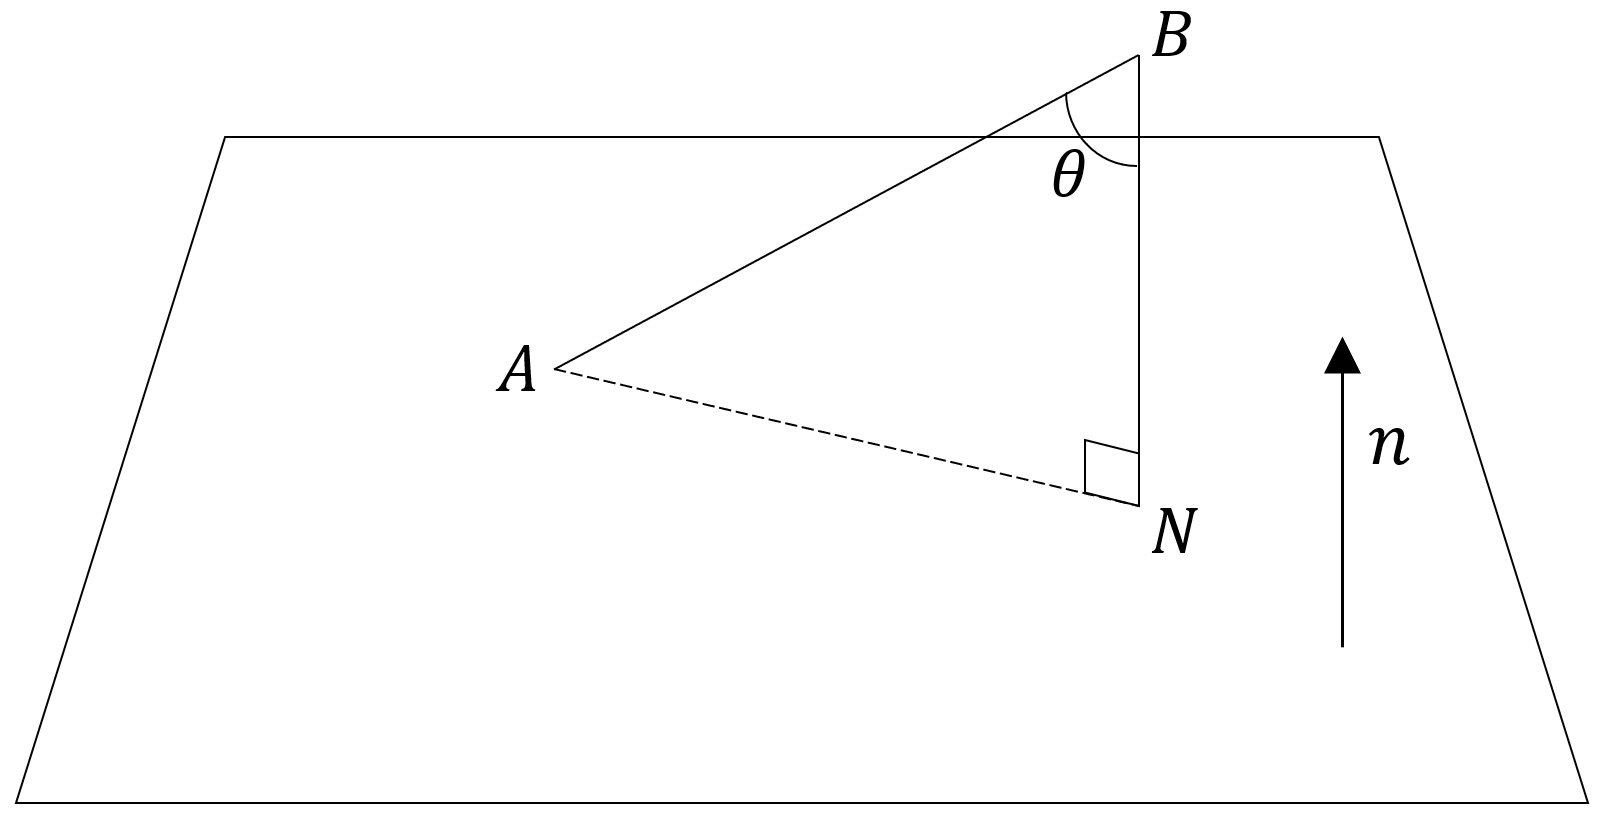
\includegraphics[width=\textwidth]{pointfromplane}}
\end{figure}
$\overrightarrow{AB}=\boldsymbol{b}-\boldsymbol{a}$, and from simple geometry,
\begin{equation*}
\left|\overrightarrow{BN}\right|=|\boldsymbol{b}-\boldsymbol{a}|\cos(\theta)
\end{equation*}
We can then use the scalar product theorem and rearrange:
\begin{align*}
(\boldsymbol{b}-\boldsymbol{a})\cdot\boldsymbol{n}&=|\boldsymbol{b}-\boldsymbol{a}||\boldsymbol{n}|\cos(\theta) \\
\frac{\left| (\boldsymbol{b}-\boldsymbol{a})\cdot\boldsymbol{n} \right|}{|\boldsymbol{n}|}&=|\boldsymbol{b}-\boldsymbol{a}|\cos(\theta)=\left|\overrightarrow{BN}\right|
\end{align*}
\scriptsize
Since $0\leq\theta\leq\frac{\pi}{2}$, $0\leq\cos(\theta)\leq1$. Therefore, $|\boldsymbol{b}-\boldsymbol{a}|\cos(\theta)>0$, so the modulus of $(\boldsymbol{b}-\boldsymbol{a})\cdot\boldsymbol{n}$ must be taken.
\normalsize

\begin{equation*}
\left| (\boldsymbol{b}-\boldsymbol{a})\cdot\boldsymbol{n} \right|=\left| \boldsymbol{b}\cdot\boldsymbol{n}-\boldsymbol{a}\cdot\boldsymbol{n} \right|
\end{equation*}
And recall that $\boldsymbol{a}$ is an arbitrary point in the plane. using the fact that $\boldsymbol{a}\cdot\boldsymbol{n}=p$, we can substitute in:
\begin{equation*}
\left| (\boldsymbol{b}-\boldsymbol{a})\cdot\boldsymbol{n} \right|=\left| \boldsymbol{b}\cdot\boldsymbol{n}-p \right|
\end{equation*}
Therefore
\begin{equation*}
\left|\overrightarrow{BN}\right|=\frac{\left| \boldsymbol{b}\cdot\boldsymbol{n}-p \right|}{|\boldsymbol{n}|}
\end{equation*}


\vspace{0.5cm}
\subsubsection*{The distance of a point from a line}
$A$ and $N$ are points (with vectors $\boldsymbol{a}$ and $\boldsymbol{n}$ respectively) contained within the line defined by $\boldsymbol{r}=\boldsymbol{a}+\lambda\boldsymbol{n}$. $\overrightarrow{NB}$ is such that it is perpendicular to the line. $B$ is a point in space (with vector $\boldsymbol{b}$), and $\boldsymbol{n}$ is a vector parallel to the line.
\begin{figure}[H]
\centering
\scalebox{.65}{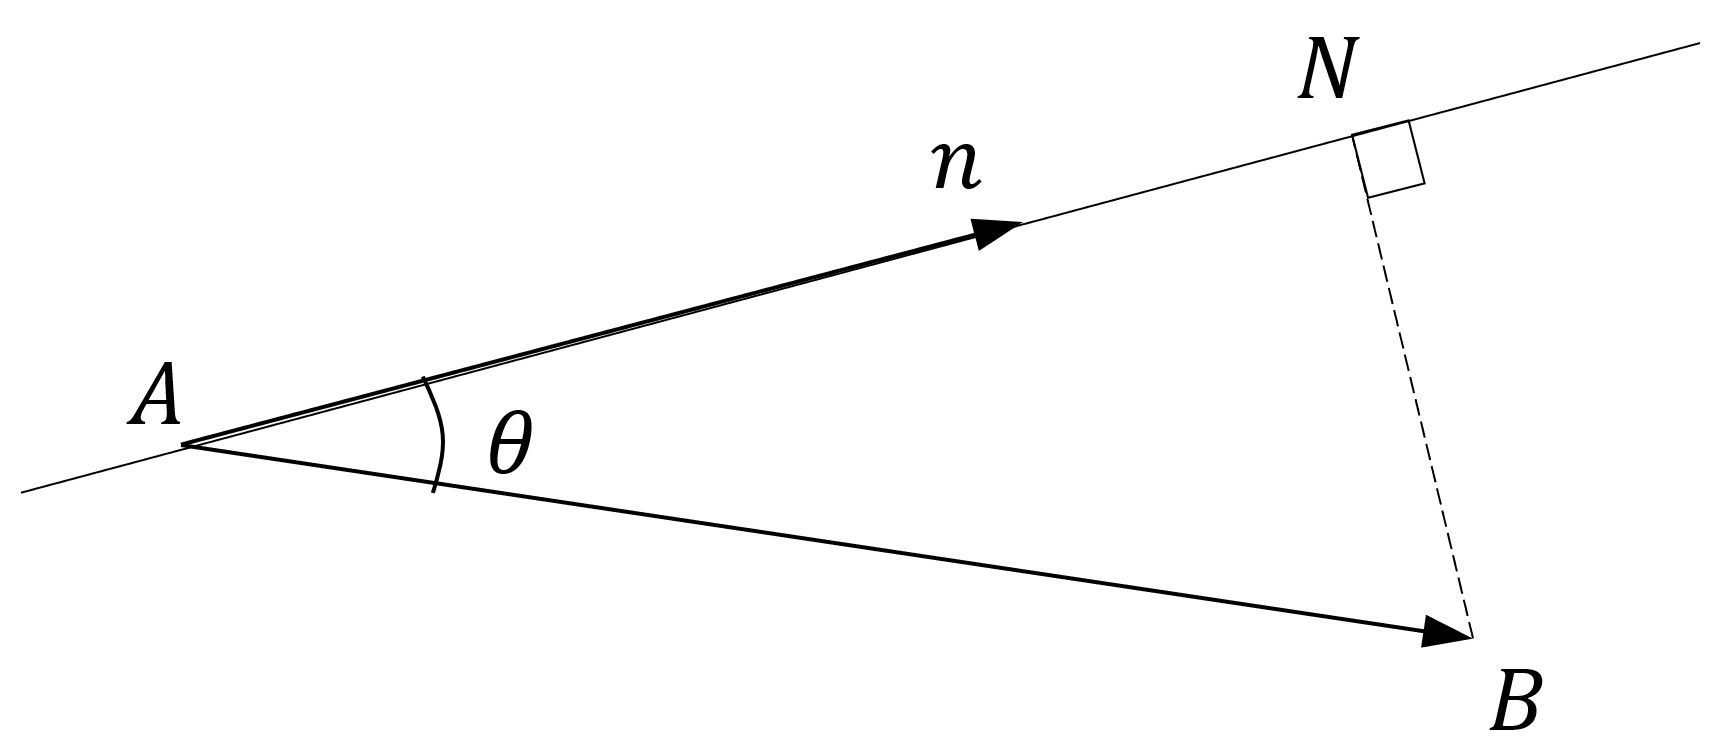
\includegraphics[width=\textwidth]{pointfromline}}
\end{figure}
$\overrightarrow{AB}=\boldsymbol{b}-\boldsymbol{a}$, and from simple geometry,
\begin{equation*}
\left|\overrightarrow{BN}\right|=|\boldsymbol{b}-\boldsymbol{a}|\sin(\theta)
\end{equation*}
We can then use the vector product theorem and rearrange:
\begin{align*}
(\boldsymbol{b}-\boldsymbol{a})\times\boldsymbol{n}&=|\boldsymbol{b}-\boldsymbol{a}||\boldsymbol{n}|\sin(\theta) \\
\frac{\left| (\boldsymbol{b}-\boldsymbol{a})\times\boldsymbol{n} \right|}{|\boldsymbol{n}|}&=|\boldsymbol{b}-\boldsymbol{a}|\sin(\theta)=\left|\overrightarrow{BN}\right|
\end{align*}
\scriptsize
Since $0\leq\theta\leq\frac{\pi}{2}$, $0\leq\sin(\theta)\leq1$. Therefore, $|\boldsymbol{b}-\boldsymbol{a}|\sin(\theta)>0$, so the modulus of $(\boldsymbol{b}-\boldsymbol{a})\times\boldsymbol{n}$ must be taken.
\normalsize

\subsubsection*{The distance of a point from a line in 2D}
Consider a line defined by
\begin{equation*}
ax+by=c
\end{equation*}
and the point $(x_{1},y_{1})$ in the $x$--$y$ plane, embedded in 3D space. \newline \par

The axis intercepts are $\left(\frac{c}{a},0,0\right)$ and $\left(0,\frac{c}{b},0\right)$. Therefore a vector equation of the line is given by
\begin{equation*}
\boldsymbol{r}=\begin{bmatrix} \frac{c}{a} \\ 0 \\ 0 \end{bmatrix}+\lambda\begin{bmatrix} \frac{c}{a} \\ -\frac{c}{b} \\ 0 \end{bmatrix}
\end{equation*}
Hence the distance of a point $\begin{bmatrix}x_{1} \\ y_{1} \\ 0 \end{bmatrix}$ from the line is
\small
\begin{align*}
\frac{\left| (\boldsymbol{b}-\boldsymbol{a})\times\boldsymbol{n} \right|}{|\boldsymbol{n}|}&=\frac{\left| \left(\begin{bmatrix}x_{1} \\ y_{1} \\ 0 \end{bmatrix}-\begin{bmatrix} \frac{c}{a} \\ 0 \\ 0 \end{bmatrix}\right)\times\begin{bmatrix} \frac{c}{a} \\ -\frac{c}{b} \\ 0 \end{bmatrix} \right|}{\left|\begin{bmatrix} \frac{c}{a} \\ -\frac{c}{b} \\ 0 \end{bmatrix}\right|}&=\frac{\left| \begin{bmatrix}x_{1}-\frac{c}{a} \\ y_{1} \\ 0 \end{bmatrix}\times\begin{bmatrix} \frac{c}{a} \\ -\frac{c}{b} \\ 0 \end{bmatrix} \right|}{\left|\begin{bmatrix} \frac{c}{a} \\ -\frac{c}{b} \\ 0 \end{bmatrix}\right|} \\
&=\frac{\left| \begin{bmatrix}0 \\ 0 \\ -\frac{x_{1}c}{b}+\frac{c^{2}}{ab}-\frac{y_{1}c}{a} \end{bmatrix} \right|}{\left|\begin{bmatrix} \frac{c}{a} \\ -\frac{c}{b} \\ 0 \end{bmatrix}\right|} &=\frac{\left| \begin{bmatrix}0 \\ 0 \\ \frac{c\left( c-x_{1}a-y_{1}b \right)}{ab} \end{bmatrix} \right|}{\left|\begin{bmatrix} \frac{c}{a} \\ -\frac{c}{b} \\ 0 \end{bmatrix}\right|} \\ 
&=\frac{\sqrt{\frac{c^{2}\left( c-x_{1}a-y_{1}b \right)^{2}}{(ab)^{2}}}}{\sqrt{\left( \frac{c}{a} \right)^{2} + \left( \frac{c}{b} \right)^{2}}} &=\frac{\frac{c}{ab}\sqrt{\left( c-x_{1}a-y_{1}b \right)^{2}}}{\frac{c}{ab}\sqrt{a^{2}+b^{2}}} \\
&=\frac{\left| c-x_{1}a-y_{1}b \right|}{\sqrt{a^{2}+b^{2}}} &=\frac{\left| x_{1}a+y_{1}b-c \right|}{\sqrt{a^{2}+b^{2}}}
\end{align*}
\normalsize
\vspace{0.5cm}


\subsection{The volume of a parallelepiped and the scalar triple product}
\begin{figure}[H]
\centering
\scalebox{.5}{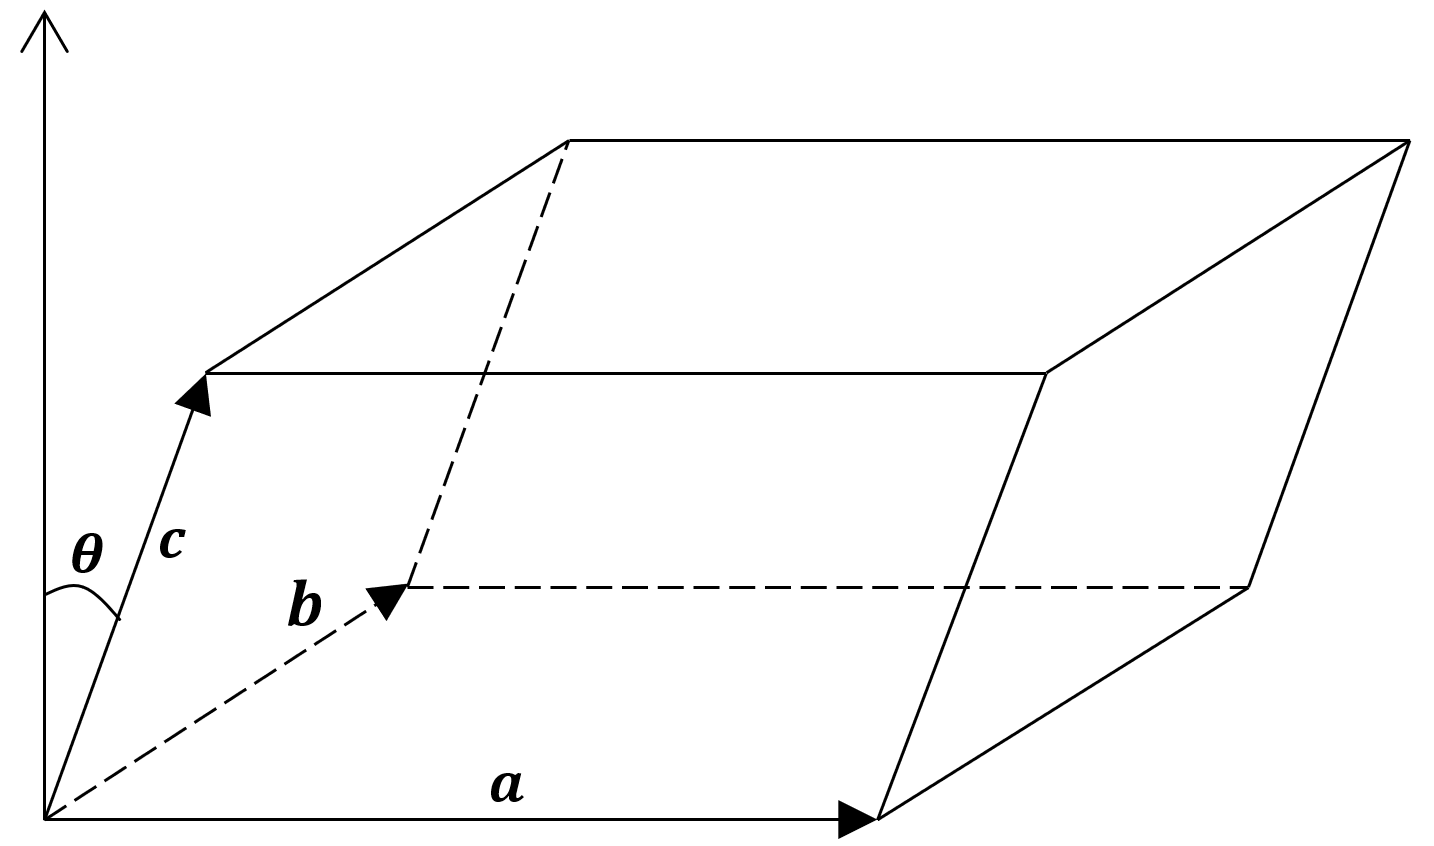
\includegraphics[width=\textwidth]{parallelepiped}}
\end{figure}
For a parallelepiped defined by the vectors $\boldsymbol{a}$, $\boldsymbol{b}$, and $\boldsymbol{c}$, the base area is defined by $\left|\boldsymbol{a}\times\boldsymbol{b}\right|$, and the perpendicular height is $\left|\boldsymbol{c}\right|\cos(\theta)$. \newline \par

Therefore the volume of the parallelepiped is
\begin{equation*}
\left|\boldsymbol{a}\times\boldsymbol{b}\right|\cdot\left|\boldsymbol{c}\right|\cos(\theta)=(\boldsymbol{a}\times\boldsymbol{b})\cdot\boldsymbol{c}
\end{equation*}
This is called the \emph{scalar triple product} of the vectors $\boldsymbol{a}$, $\boldsymbol{b}$, and $\boldsymbol{c}$. The result gives the signed volume of the parallelepiped spanned by $\boldsymbol{a}$, $\boldsymbol{b}$, and $\boldsymbol{c}$. So, in the case of a $3\times3$ matrix, this gives the volume scale factor of the unit cube, if $\boldsymbol{a}$, $\boldsymbol{b}$, and $\boldsymbol{c}$ are the three vectors that comprise the matrix. \newline \par

The scalar triple product has a cyclic property;
\begin{equation*}
\boldsymbol{c}\cdot(\boldsymbol{a}\times\boldsymbol{b})\equiv\boldsymbol{b}\cdot(\boldsymbol{c}\times\boldsymbol{a})\equiv\boldsymbol{a}\cdot(\boldsymbol{b}\times\boldsymbol{c})
\end{equation*}
since the scalar triple product is invariant under a circular shift of the vectors. \newline\par

$\boldsymbol{a}\cdot(\boldsymbol{b}\times\boldsymbol{c})$ is positive when $\boldsymbol{a}$, $\boldsymbol{b}$, and $\boldsymbol{c}$ form a right - handed set, and negative when $\boldsymbol{a}$, $\boldsymbol{b}$, and $\boldsymbol{c}$ form a left - handed set.
\vspace{0.5cm}
\newpage
\subsection{Configurations of three planes in three dimensions}
\begin{itemize}
\item A Level FM Year 2 \hspace{1cm} \phantom{AS /} Pages 104 -- 110
\end{itemize} \par
There are eight possible configurations of three planes in three dimensions. Given three planes, you should be able to establish which configuration they fall into, and find the point, line, or plane of solutions. An example system of planes / equations for each of the eight configuration is given in section \ref{planesexamples}

\begin{center}
\small
\begin{tblr}{|[1pt]|c|l|c|c||[1pt]}
\hline[1pt]
\# & Description & Nature of solutions & $\hspace{1cm}\text{Sketch}\hspace{1cm}$ \\ \hline[1pt]
\SetCell[r=1,c=4]{c} $\det\boldsymbol{M}\neq0$ \\ \hline[1pt]
\SetCell[r=2,c=1]{c}1&\SetCell[r=2,c=1]{l}\begin{tabular}{l}Planes intersect at a \\single point\end{tabular} & \SetCell[r=2,c=1]{c}Unique solution & \SetCell[r=2,c=1]{c}\scalebox{.1}{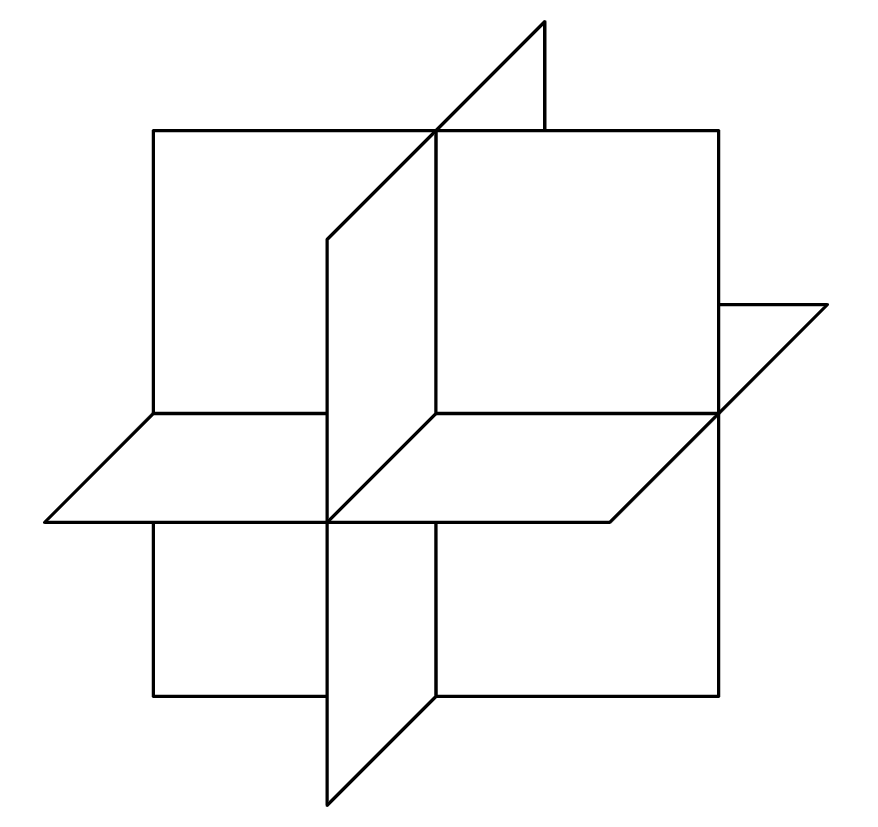
\includegraphics[width=\textwidth]{planeintersection1}} \\
& & & \\ \hline[1pt]
\SetCell[r=1,c=4]{c} $\det\boldsymbol{M}=0$ \\ \hline[1pt]
\SetCell[r=2,c=1]{c}2&\SetCell[r=2,c=1]{l}\begin{tabular}{l}Planes all parallel and \\none coincident\\\end{tabular} & \SetCell[r=8,c=1]{c}No solutions & \SetCell[r=2,c=1]{c}\scalebox{.25}{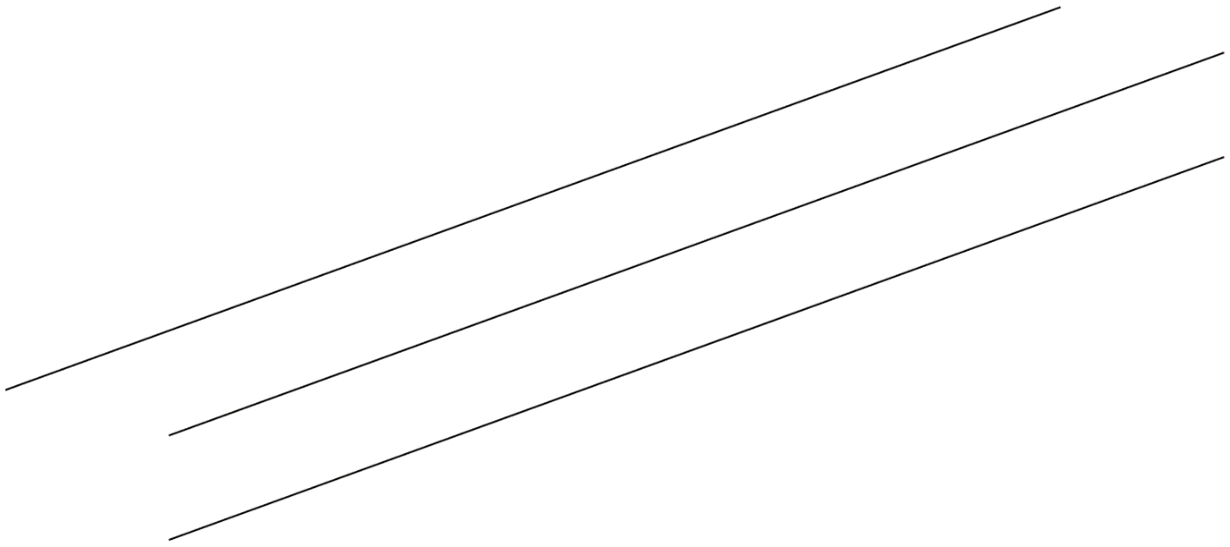
\includegraphics[width=\textwidth]{planeintersection21}} \\
& & & \\ \hline
\SetCell[r=2,c=1]{c}3&\SetCell[r=2,c=1]{l}\begin{tabular}{l}Planes all parallel and \\ only two coincident\end{tabular} &  & \SetCell[r=2,c=1]{c}\scalebox{.25}{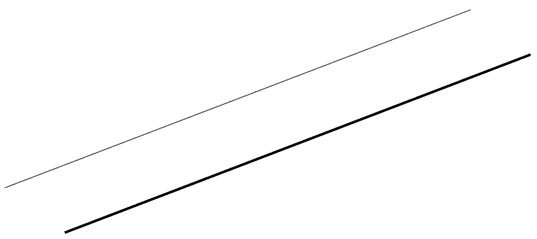
\includegraphics[width=\textwidth]{planeintersection31}} \\
& & & \\ \hline
\SetCell[r=2,c=1]{c}4&\SetCell[r=2,c=1]{l}\begin{tabular}{l}Two planes parallel but \\ non-coincident, with \\one traversing\end{tabular} &  & \SetCell[r=2,c=1]{c}\scalebox{.25}{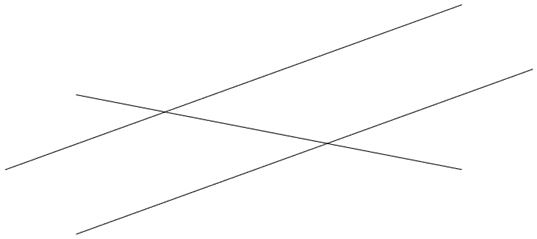
\includegraphics[width=\textwidth]{planeintersection41}} \\
& & & \\ \hline
\SetCell[r=2,c=1]{c}5&\SetCell[r=2,c=1]{l}\begin{tabular}{l}Planes intersect to form \\a triangular prism\end{tabular} &  & \SetCell[r=2,c=1]{c}\scalebox{.25}{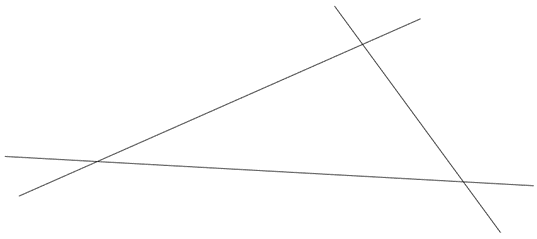
\includegraphics[width=\textwidth]{planeintersection51}} \\
& & & \\ \hline[1pt]
\SetCell[r=2,c=1]{c}6&\SetCell[r=2,c=1]{l}\begin{tabular}{l}Planes form a sheaf\end{tabular} & \SetCell[r=4,c=1]{c}Line of solutions & \SetCell[r=2,c=1]{c}\scalebox{.25}{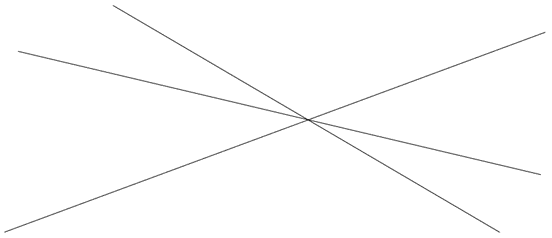
\includegraphics[width=\textwidth]{planeintersection61}} \\
& & & \\ \hline
\SetCell[r=2,c=1]{c}7&\SetCell[r=2,c=1]{l}\begin{tabular}{l}Two planes coincident \\with one traversing\end{tabular} &  & \SetCell[r=2,c=1]{c}\scalebox{.25}{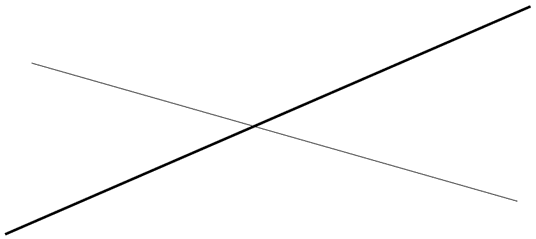
\includegraphics[width=\textwidth]{planeintersection71}} \\
& & & \\ \hline[1pt]
\SetCell[r=2,c=1]{c}8&\SetCell[r=2,c=1]{l}\begin{tabular}{l}Three planes coincident\end{tabular} & \SetCell[r=2,c=1]{c}Plane of solutions & \SetCell[r=2,c=1]{c}\scalebox{.25}{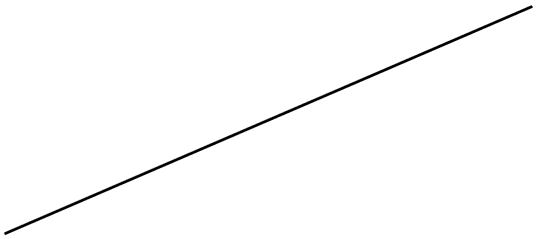
\includegraphics[width=\textwidth]{planeintersection81}} \\ 
& & & \\ \hline[1pt]
\end{tblr}
\end{center}
\normalsize
\vspace{0.5cm}

\newpage
\subsection{Examples of configurations of three planes in three dimensions}
\label{planesexamples}
\begin{itemize}
\item A Level FM Year 2 \hspace{1cm} \phantom{AS /} Pages 104 -- 110
\end{itemize} \par
\begin{center}
\scriptsize
\begin{tblr}{|[1pt]|c|c|c|c||[1pt]}
\hline[1pt]
\# & System & Matrix equation & Nature of solution\\ \hline[1pt]
\SetCell[r=1,c=4]{c} $\det\boldsymbol{M}\neq0$ \\ \hline[1pt]
\SetCell[r=2,c=1]{c}1&\SetCell[r=2,c=1]{c} \parbox{1cm}{\vspace{-.4cm}\begin{align*}
4x-\phantom{3}y-\phantom{4}z&=17\\
x+\phantom{3}y-4z&=3\\
2x-3y+2z&=6 
\end{align*}\vspace{-.4cm}}& \SetCell[r=2,c=1]{c} $\begin{bmatrix}4&-1&-1\\1&\phantom{-}1&-4\\2&-3&\phantom{-}2\end{bmatrix}\begin{bmatrix}x\\y\\z\end{bmatrix}=\begin{bmatrix}17\\3\\6\end{bmatrix}$ & \SetCell[r=2,c=1]{c} \parbox{3cm}{\vspace{-.4cm}Planes intersect at a single point\vspace{-.4cm}} \\
& & & \\ \hline[1pt]
\SetCell[r=1,c=4]{c} $\det\boldsymbol{M}=0$ \\ \hline[1pt]
\SetCell[r=2,c=1]{c}2&\SetCell[r=2,c=1]{c}\parbox{1cm}{\vspace{-.4cm}\begin{align*}
2x-2y+4z&=20\\
3x-3y+6z&=24\\
x-\phantom{3}y+2z&=5 
\end{align*}\vspace{-.4cm}} & \SetCell[r=2,c=1]{c} $\begin{bmatrix}2&-2&\phantom{-}4\\3&-3&\phantom{-}6\\1&-1&\phantom{-}2\end{bmatrix}\begin{bmatrix}x\\y\\z\end{bmatrix}=\begin{bmatrix}20\\24\\5\end{bmatrix}$ & \SetCell[r=2,c=1]{c} \parbox{3cm}{\vspace{-.4cm}Planes all parallel and none coincident\vspace{-.4cm}} \\
& & & \\ \hline
\SetCell[r=2,c=1]{c}3&\SetCell[r=2,c=1]{c}\parbox{1cm}{\vspace{-.4cm}\begin{align*}
2x-2y+4z&=20\\
3x-3y+6z&=15\\
x-\phantom{3}y+2z&=5 
\end{align*}\vspace{-.4cm}}& \SetCell[r=2,c=1]{c} $\begin{bmatrix}2&-2&\phantom{-}4\\3&-3&\phantom{-}6\\1&-1&\phantom{-}2\end{bmatrix}\begin{bmatrix}x\\y\\z\end{bmatrix}=\begin{bmatrix}20\\15\\5\end{bmatrix}$ & \SetCell[r=2,c=1]{c} \parbox{3cm}{\vspace{-.4cm}Planes all parallel and only two coincident\vspace{-.4cm}} \\
& & & \\ \hline
\SetCell[r=2,c=1]{c}4&\SetCell[r=2,c=1]{c} \parbox{1cm}{\vspace{-.4cm}\begin{align*}
2x-2y+4z&=20\\
3x-3y+6z&=15\\
2x-3y+2z&=6 
\end{align*}\vspace{-.4cm}}& \SetCell[r=2,c=1]{c} $\begin{bmatrix}2&-2&\phantom{-}4\\3&-3&\phantom{-}6\\2&-3&\phantom{-}2\end{bmatrix}\begin{bmatrix}x\\y\\z\end{bmatrix}=\begin{bmatrix}20\\15\\6\end{bmatrix}$ & \SetCell[r=2,c=1]{c} \parbox{3cm}{\vspace{-.4cm}Two planes parallel but non-coincident, with one traversing\vspace{-.4cm}} \\
& & & \\ \hline
\SetCell[r=2,c=1]{c}5&\SetCell[r=2,c=1]{c} \parbox{1cm}{\vspace{-.4cm}\begin{align*}
4x-y-\phantom{4}z&=17\\
x+y-4z&=3\\
x-y+2z&=11
\end{align*}\vspace{-.4cm}}& \SetCell[r=2,c=1]{c} $\begin{bmatrix}4&-1&-1\\1&\phantom{-}1&-4\\1&-1&\phantom{-}2\end{bmatrix}\begin{bmatrix}x\\y\\z\end{bmatrix}=\begin{bmatrix}17\\3\\11\end{bmatrix}$ & \SetCell[r=2,c=1]{c} \parbox{3cm}{\vspace{-.4cm}Planes intersect to form a triangular prism\vspace{-.4cm}} \\
& & & \\ \hline[1pt]
\SetCell[r=2,c=1]{c}6&\SetCell[r=2,c=1]{c} \parbox{1cm}{\vspace{-.4cm}\begin{align*}
4x-y-\phantom{4}z&=17\\
x+y-4z&=3\\
x-y+2z&=5 
\end{align*}\vspace{-.4cm}}& \SetCell[r=2,c=1]{c} $\begin{bmatrix}4&-1&-1\\1&\phantom{-}1&-4\\1&-1&\phantom{-}2\end{bmatrix}\begin{bmatrix}x\\y\\z\end{bmatrix}=\begin{bmatrix}17\\3\\5\end{bmatrix}$ & \SetCell[r=2,c=1]{c} \parbox{3cm}{\vspace{-.4cm}Planes form a sheaf\vspace{-.4cm}} \\
& & & \\ \hline
\SetCell[r=2,c=1]{c}7&\SetCell[r=2,c=1]{c} \parbox{1cm}{\vspace{-.4cm}\begin{align*}
2x-2y+4z&=10\\
3x-3y+6z&=15\\
2x-3y+2z&=6 
\end{align*}\vspace{-.4cm}}& \SetCell[r=2,c=1]{c} $\begin{bmatrix}2&-2&\phantom{-}4\\3&-3&\phantom{-}6\\2&-3&\phantom{-}2\end{bmatrix}\begin{bmatrix}x\\y\\z\end{bmatrix}=\begin{bmatrix}10\\15\\6\end{bmatrix}$ & \SetCell[r=2,c=1]{c} \parbox{3cm}{\vspace{-.4cm}Two planes coincident with one traversing\vspace{-.4cm}} \\
& & & \\ \hline[1pt]
\SetCell[r=2,c=1]{c}8&\SetCell[r=2,c=1]{c} \parbox{1cm}{\vspace{-.4cm}\begin{align*}
2x-2y+4z&=10\\
3x-3y+6z&=15\\
x-\phantom{3}y+2z&=5 
\end{align*}\vspace{-.4cm}}& \SetCell[r=2,c=1]{c} $\begin{bmatrix}2&-2&\phantom{-}4\\3&-3&\phantom{-}6\\1&-1&\phantom{-}2\end{bmatrix}\begin{bmatrix}x\\y\\z\end{bmatrix}=\begin{bmatrix}10\\15\\5\end{bmatrix}$ & \SetCell[r=2,c=1]{c} \parbox{3cm}{\vspace{-.4cm}Three planes coincident\vspace{-.4cm}} \\
& & & \\ \hline[1pt]
\end{tblr}
\end{center}
\vspace{0.25cm}

\newpage
\subsection{Linear transformations - matrices}
\begin{itemize}
\item A Level FM AS / Year 1 \hspace{1cm} Pages 1 -- 7
\item A Level FM AS / Year 1 \hspace{1cm} Pages 71 -- 94
\item A Level FM Year 2 \hspace{1cm} \phantom{AS /} Pages 101 -- 104
\end{itemize} \par

Linear transformations map points from one to another, and can be represented by matrices.
\begin{equation*}
\begin{bmatrix} a & b \\ c& d\end{bmatrix}\begin{bmatrix} x \\ y \end{bmatrix}=\begin{bmatrix} ax+by \\ cx+dy\end{bmatrix}
\end{equation*}
\begin{itemize}
\item[-]Linear transformations maintain parallel lines, though perpendicular lines may not always be maintained.
\item[-]The origin $(0,0)$ is \emph{always} mapped onto itself by a linear transformation.
	\item[-]Using matrix $\boldsymbol{A}$ and then $\boldsymbol{B}$, where $\boldsymbol{A}=\begin{bmatrix} a & b \\ c& d\end{bmatrix}$, and $\boldsymbol{B}=\begin{bmatrix} p & q \\ r & s \end{bmatrix}$, on $\begin{bmatrix} x \\ y \end{bmatrix}$ is represented as $\boldsymbol{BA}\begin{bmatrix} x\\ y\end{bmatrix}$, and the matrix $\boldsymbol{BA}$ is
\begin{equation*}
\boldsymbol{BA}=\begin{bmatrix} p & q \\ r& s\end{bmatrix}\begin{bmatrix} a & b \\ c& d\end{bmatrix}=\begin{bmatrix} pa+qc & pb+qd \\ ra+sc& rb+sd\end{bmatrix}
\end{equation*}
\item[-]The identity matrix is 
\begin{equation*}
\begin{bmatrix} 1 & 0 \\ 0& 1\end{bmatrix}
\end{equation*}
and maps every point to itself. Its algebraic equivalent is multiplying by 1.
The first column of a matrix is where the vector $\hat{\boldsymbol{\imath}}$ maps to. The second column is where the vector $\hat{\boldsymbol{\jmath}}$ maps to. For a three-dimensional matrix, the third column is where the vector $\hat{\boldsymbol{k}}$ maps to.
\item[-]A $2\times2$ anticlockwise rotation matrix of an angle $\theta$ has the form
\begin{equation*}
\begin{bmatrix} \cos(\theta) & -\sin(\theta) \\ \sin(\theta) & \cos(\theta) \end{bmatrix}
\end{equation*}
\item[-] Linear transformations include \emph{reflections}, \emph{rotations}, \emph{enlargements}, and \emph{shears}, or can be a combination of any of them
\item[-] \textbf{\underline{Invariant lines}} are lines which do not move under the transformation
\item[-] \textbf{\underline{Invariant points}} are points which do not move under the transformation
\end{itemize} \par
\vspace{0.5cm}

\subsection{Standard matrices}
\begin{itemize}
\item A Level FM AS / Year 1 \hspace{1cm} Pages 81 -- 82
\item A Level FM AS / Year 1 \hspace{1cm} Pages 90 -- 91
\end{itemize} \par
The $2\times2$ matrices you should recognise are listed below.
\scriptsize
\begin{center}
\begin{tblr}{|[.75pt]|l|cc|c||[.75pt]}
\hline[1pt]
Transformation & \SetCell[r=1,c=2]{c} Matrix & &Determinant \\ \hline[.75pt]
\SetCell[r=2,c=1]{l} \parbox{3cm}{Anticlockwise rotation about $O$, angle $\theta$} & \SetCell[r=2,c=2]{c}$\begin{bmatrix}\cos(\theta) & -\sin(\theta) \\ \sin(\theta)&\cos(\theta)\end{bmatrix}$ & &\SetCell[r=2,c=1]{c}1 \\
& & & \\ \hline
\SetCell[r=2,c=1]{l} \parbox{3cm}{Reflection in coordinate axes} & \SetCell[r=2,c=1]{c}\parbox{1.5cm}{\vspace{-.5cm}\begin{gather*}x\text{-axis} \\ \begin{bmatrix}1 & 0 \\ 0&-1\end{bmatrix}\end{gather*}\vspace{-.4cm}}& \SetCell[r=2,c=1]{c}\parbox{1.5cm}{\vspace{-.5cm}\begin{gather*}y\text{-axis} \\ \begin{bmatrix}-1 & 0 \\ 0&1\end{bmatrix}\end{gather*}\vspace{-.4cm}} & \SetCell[r=2,c=1]{c}-1 \\
& & & \\ \hline
\SetCell[r=2,c=1]{l} \parbox{3cm}{Reflection in the lines $y=\pm x$} & \SetCell[r=2,c=2]{c}$\begin{bmatrix}0 & \pm1 \\ \pm1&0\end{bmatrix}$ & &\SetCell[r=2,c=1]{c}-1 \\
& & & \\ \hline
\SetCell[r=2,c=1]{l} \parbox{3cm}{Stretch, scale factor $c$, with the $y$-axis invariant} & \SetCell[r=2,c=2]{c}$\begin{bmatrix}c & 0 \\ 0&1\end{bmatrix}$ & &\SetCell[r=2,c=1]{c}$c$ \\
& & & \\ \hline
\SetCell[r=2,c=1]{l} \parbox{3cm}{Stretch, scale factor $d$, with the $x$-axis invariant} & \SetCell[r=2,c=2]{c}$\begin{bmatrix}1 & 0 \\ 0&d\end{bmatrix}$ & &\SetCell[r=2,c=1]{c}$d$ \\
& & & \\ \hline
\SetCell[r=2,c=1]{l} \parbox{3cm}{Enlargement, centre $O$, scale factor $k$} & \SetCell[r=2,c=2]{c}$\begin{bmatrix}k & 0 \\ 0&k\end{bmatrix}$ & &\SetCell[r=2,c=1]{c}$k^{2}$ \\
& & & \\ \hline
\SetCell[r=2,c=1]{l} \parbox{3cm}{Shear, $x$-axis invariant,\\$(0,1)\rightarrow(k,1)$} & \SetCell[r=2,c=2]{c}$\begin{bmatrix}1 & k \\ 0&1\end{bmatrix}$ & &\SetCell[r=2,c=1]{c}1 \\
& & & \\ \hline
\SetCell[r=2,c=1]{l} \parbox{3cm}{Shear, $y$-axis invariant,\\$(1,0)\rightarrow(1,k)$} & \SetCell[r=2,c=2]{c}$\begin{bmatrix}1 & 0 \\ k&1\end{bmatrix}$ & &\SetCell[r=2,c=1]{c}1 \\
& & & \\ \hline[.75pt]
\end{tblr}
\end{center}
\normalsize
\par The $3\times3$ matrices you should recognise are reflections along the $x$-$y$, $x$-$z$, and $y$-$z$ planes, and rotations about each axis. Here are the anticlockwise rotations, followed by the reflections.
\begin{center}
\begin{tblr}{|[.75pt]|c|c|c||[.75pt]}
\hline[1pt]
$y$-$z$ plane ($x=0$) & $x$-$z$ plane ($y=0$) & $x$-$y$ plane ($z=0$) \\ \hline[.75pt]
$\begin{bmatrix} -1 & 0 & 0 \\ 0 & 1 & 0 \\ 0 & 0 & 1 \end{bmatrix}$ &
$\begin{bmatrix} 1 & 0 & 0 \\ 0 & -1 & 0 \\ 0 & 0 & 1 \end{bmatrix}$ &
$\begin{bmatrix} 1 & 0 & 0 \\ 0 & 1 & 0 \\ 0 & 0 & -1 \end{bmatrix}$ \\ \hline[.75pt]
\end{tblr}
\end{center}
\begin{center}
\begin{tblr}{|[.75pt]|c|c|c||[.75pt]}
\hline[1pt]
$x$-axis & $y$-axis & $z$-axis \\ \hline[.75pt]
$\begin{bmatrix} 1 & 0 & 0 \\ 0 & \cos(\theta) & -\sin(\theta) \\ 0 & \sin(\theta) & \cos(\theta) \end{bmatrix}$ &
$\begin{bmatrix} \cos(\theta) & 0 & \sin(\theta) \\ 0 & 1 & 0 \\ -\sin(\theta) & 0 & \cos(\theta) \end{bmatrix}$ &
$\begin{bmatrix} \cos(\theta) & -\sin(\theta) & 0 \\ \sin(\theta) & \cos(\theta) & 0 \\ 0 & 0 & 1 \end{bmatrix}$ \\ \hline[.75pt]
\end{tblr}
\end{center}
\vspace{0.5cm}

\newpage

\subsection{Matrix multiplication}
\begin{itemize}
\item A Level FM AS / Year 1 \hspace{1cm} Pages 7 -- 13
\end{itemize} \par
To multiply two matrices together, multiply the rows of the first matrix by columns of a second matrix. Two matrices can be multiplied if the number of columns in matrix $\boldsymbol{A}$ is equal to the number of rows in matrix $\boldsymbol{B}$. So if a $m\times n$ matrix multiplies an $n\times p$ matrix, the result is a $m\times p$ matrix.
\begin{equation*}
\begin{bmatrix}\cdot&\cdot&\cdot\\\cdot&\cdot&\cdot\\\cdot&\cdot&\cdot\\\cdot&\cdot&\cdot\end{bmatrix}\times\begin{bmatrix}\cdot&\cdot&\cdot&\cdot&\cdot\\\cdot&\cdot&\cdot&\cdot&\cdot\\\cdot&\cdot&\cdot&\cdot&\cdot\end{bmatrix}=\begin{bmatrix}\cdot&\cdot&\cdot&\cdot&\cdot\\\cdot&\cdot&\cdot&\cdot&\cdot\\\cdot&\cdot&\cdot&\cdot&\cdot\\\cdot&\cdot&\cdot&\cdot&\cdot\end{bmatrix}
\end{equation*}
\vspace{0.5cm}


\subsection{Determinant of a 2$\,\times\,$2 matrix}
\begin{itemize}
\item A Level FM AS / Year 1 \hspace{1cm} Pages 13 -- 23
\end{itemize} \par
For a matrix $\boldsymbol{M}=\begin{bmatrix}a&b\\c&d\end{bmatrix}$, the determinant is defined by
\begin{equation*}
\det \boldsymbol{M}=\det\begin{bmatrix}a&b\\c&d\end{bmatrix}=ad-bc
\end{equation*}
The determinant gives an area\footnote{volume in the case of a $3\times3$ matrix} scale factor of the matrix. \newline\par
If the determinant is negative, then it implies an inversion of the points (if points are $ABCD$ clockwise originally, then after matrix transformation, they will read $ADCB$ clockwise) \newline\par
If the determinant is $0$, then the matrix collapses space onto a line, or a point if $\boldsymbol{M}=\begin{bmatrix}0&0\\0&0\end{bmatrix}$
\begin{itemize}
\item[Note:] \begin{equation*}
\det \boldsymbol{MN}=\det \boldsymbol{M}\times\det \boldsymbol{N}
\end{equation*}
\end{itemize}
\vspace{0.5cm}

\newpage
\subsection{Inverse of a 2$\,\times\,$2 matrix}
\label{2x2inverse}
\begin{itemize}
\item A Level FM AS / Year 1 \hspace{1cm} Pages 13 -- 23
\end{itemize} \par
The inverse of a matrix $\boldsymbol{M}=\begin{bmatrix}a&b\\c&d\end{bmatrix}$ is defined by 
\begin{equation*}
\boldsymbol{M}^{-1}=\frac{1}{\det \boldsymbol{M}}\begin{bmatrix}d&-b\\-c&a\end{bmatrix}=\begin{bmatrix}\frac{d}{ad-bc}&\frac{-b}{ad-bc}\\\frac{-c}{ad-bc}&\frac{a}{ad-bc}\end{bmatrix}
\end{equation*} \newline \par
We can use the inverse of a matrix to solve a pair of simultaneous equations. Given the equations
\begin{equation*}
\begin{Bmatrix}2x+y=4 \\ 3x+4y=11 \end{Bmatrix}
\end{equation*}
These can be represented by the matrix equation
\begin{equation*}
\begin{bmatrix}2&1\\3&4\end{bmatrix}\begin{bmatrix}x\\y\end{bmatrix}=\begin{bmatrix}4\\11\end{bmatrix}
\end{equation*}
So, by taking the inverse matrix and applying it to both sides,
\begin{align*}
\begin{bmatrix}x\\y\end{bmatrix}&=\frac{1}{2\times4-3\times1}\begin{bmatrix}4&-1\\-3&2\end{bmatrix}\begin{bmatrix}4\\11\end{bmatrix} \\
\begin{bmatrix}x\\y\end{bmatrix}&=\frac{1}{5}\begin{bmatrix} 4\times4-1\times11 \\ -3\times4+2\times11 \end{bmatrix}\\
\begin{bmatrix}x\\y\end{bmatrix}&=\frac{1}{5}\begin{bmatrix} 5 \\ 10 \end{bmatrix}\\
\begin{bmatrix}x\\y\end{bmatrix}&=\begin{bmatrix}1\\2\end{bmatrix}\\
\end{align*}
In the case that the determinant of the matrix is zero, then no unique solutions to the system exists.
\vspace{0.5cm}


\subsection{Determinant of a 3$\,\times\,$3 matrix}
\begin{itemize}
\item A Level FM AS / Year 1 \hspace{1cm} Pages 23 -- 29
\end{itemize} \par
In the same way that the determinat of a $2\times2$ matrix is the signed scale factor of the transformed unit square defined by $\hat{\boldsymbol{\imath}}$ and $\hat{\boldsymbol{\jmath}}$, the determinant of a $3\times3$ matrix is the signed volume scale factor of the transformed unit cube defined by $\hat{\boldsymbol{\imath}}$, $\hat{\boldsymbol{\jmath}}$ and $\hat{\boldsymbol{k}}$. \newline \par

Therefore if $\boldsymbol{M}=\begin{bmatrix} \uparrow & \uparrow & \uparrow \\ \boldsymbol{a} & \boldsymbol{b} & \boldsymbol{c} \\ \downarrow & \downarrow & \downarrow \end{bmatrix}$, then 
\begin{equation*}
\det\boldsymbol{M}=\boldsymbol{a}\cdot(\boldsymbol{b}\times\boldsymbol{c})=\boldsymbol{b}\cdot(\boldsymbol{c}\times\boldsymbol{a})=\boldsymbol{c}\cdot(\boldsymbol{a}\times\boldsymbol{b})
\end{equation*} (Treat the first column as a vector $\boldsymbol{a}$, the second as a vector $\boldsymbol{b}$, and the third as a vector $\boldsymbol{c}$)\newline \par

There are three cases for the determinant:
\begin{itemize}
\item[-]$\det\boldsymbol{M}>0 \hspace{.5cm}$ the transformation preserves the order of the axes (e.g. a rotation)
\item[-]$\det\boldsymbol{M}<0 \hspace{.5cm}$ the transformation reverses the order of the axes (e.g. a reflection)
\item[-]$\det\boldsymbol{M}=0 \hspace{.5cm}$ the transformation maps three dimensional space to a plane, a point, or a line.
\end{itemize}
\vspace{0.5cm}


\subsection{Inverse of a 3$\,\times\,$3 matrix}
\begin{itemize}
\item A Level FM AS / Year 1 \hspace{1cm} Pages 23 -- 29
\end{itemize} \par
For $\boldsymbol{M}=\begin{bmatrix} \uparrow & \uparrow & \uparrow \\ \boldsymbol{a} & \boldsymbol{b} & \boldsymbol{c} \\ \downarrow & \downarrow & \downarrow \end{bmatrix}=\begin{bmatrix}a_{1}&b_{1}&c_{1}\\a_{2}&b_{2}&c_{2}\\a_{3}&b_{3}&c_{3}\\ \end{bmatrix}$ and $\begin{bmatrix} \leftarrow & \boldsymbol{p} & \rightarrow \\ \leftarrow & \boldsymbol{q} & \rightarrow \\ \leftarrow & \boldsymbol{r} & \rightarrow \end{bmatrix}=\begin{bmatrix}p_{1}&p_{2}&p_{3}\\q_{1}&q_{2}&q_{3}\\r_{1}&r_{2}&r_{3}\\\end{bmatrix}$
\begin{equation*}
\begin{bmatrix} \leftarrow & \boldsymbol{p} & \rightarrow \\ \leftarrow & \boldsymbol{q} & \rightarrow \\ \leftarrow & \boldsymbol{r} & \rightarrow \end{bmatrix}\begin{bmatrix} \uparrow & \uparrow & \uparrow \\ \boldsymbol{a} & \boldsymbol{b} & \boldsymbol{c} \\ \downarrow & \downarrow & \downarrow \end{bmatrix}=\begin{bmatrix} \boldsymbol{p}\cdot\boldsymbol{a} & \boldsymbol{p}\cdot\boldsymbol{b} & \boldsymbol{p}\cdot\boldsymbol{c} \\ \boldsymbol{q}\cdot\boldsymbol{a} & \boldsymbol{q}\cdot\boldsymbol{b} & \boldsymbol{q}\cdot\boldsymbol{c} \\ \boldsymbol{r}\cdot\boldsymbol{a} & \boldsymbol{r}\cdot\boldsymbol{b} & \boldsymbol{r}\cdot\boldsymbol{c} \end{bmatrix}
\end{equation*}
And we want something of the form
\begin{equation*}
\begin{bmatrix} \leftarrow & \boldsymbol{p} & \rightarrow \\ \leftarrow & \boldsymbol{q} & \rightarrow \\ \leftarrow & \boldsymbol{r} & \rightarrow \end{bmatrix}\begin{bmatrix} \uparrow & \uparrow & \uparrow \\ \boldsymbol{a} & \boldsymbol{b} & \boldsymbol{c} \\ \downarrow & \downarrow & \downarrow \end{bmatrix}=\begin{bmatrix} ? & 0 & 0 \\ 0 & ? & 0 \\ 0 & 0 & ? \end{bmatrix}
\end{equation*}
Therefore, we need 
\begin{align*}
\boldsymbol{p}\cdot\boldsymbol{b}&=0 & \boldsymbol{p}\cdot\boldsymbol{c}&=0 & \text{Try }\boldsymbol{p}=\boldsymbol{b}\times\boldsymbol{c}\\
\boldsymbol{q}\cdot\boldsymbol{a}&=0 & \boldsymbol{q}\cdot\boldsymbol{c}&=0 & \text{Try }\boldsymbol{q}=\boldsymbol{c}\times\boldsymbol{a}\\
\boldsymbol{r}\cdot\boldsymbol{a}&=0 & \boldsymbol{r}\cdot\boldsymbol{b}&=0 & \text{Try }\boldsymbol{r}=\boldsymbol{a}\times\boldsymbol{b}
\end{align*}

Therefore
\begin{align*}
\begin{bmatrix} \leftarrow & \boldsymbol{b}\times\boldsymbol{c} & \rightarrow \\ \leftarrow & \boldsymbol{c}\times\boldsymbol{a} & \rightarrow \\ \leftarrow & \boldsymbol{a}\times\boldsymbol{b} & \rightarrow \end{bmatrix}\begin{bmatrix} \uparrow & \uparrow & \uparrow \\ \boldsymbol{a} & \boldsymbol{b} & \boldsymbol{c} \\ \downarrow & \downarrow & \downarrow \end{bmatrix}&=\begin{bmatrix} \boldsymbol{a}\cdot\boldsymbol{b}\times\boldsymbol{c} & 0 & 0 \\ 0 & \boldsymbol{b}\cdot\boldsymbol{c}\times\boldsymbol{a} & 0 \\ 0 & 0 & \boldsymbol{c}\cdot\boldsymbol{a}\times\boldsymbol{b} \end{bmatrix}\\
&=\det\boldsymbol{M}\begin{bmatrix}1&0&0\\0&1&0\\0&0&1\end{bmatrix}
\end{align*}

So
\begin{equation*}
\boldsymbol{M}^{-1}=\frac{1}{\det\boldsymbol{M}}\begin{bmatrix} \leftarrow & \boldsymbol{b}\times\boldsymbol{c} & \rightarrow \\ \leftarrow & \boldsymbol{c}\times\boldsymbol{a} & \rightarrow \\ \leftarrow & \boldsymbol{a}\times\boldsymbol{b} & \rightarrow \end{bmatrix}
\end{equation*} \newline \par

As in section \ref{2x2inverse}, we can solve a system of simultaneous equations in three variable by way of a $3\times3$ matrix. Whether or not a unique solution exists can very simply be determined by taking the determinant of the matrix that represents the system. If the determinant \emph{is} 0, then more work is required.

\vspace{0.5cm}

\end{document}